%============================================================
%  Centralized Log Management -- Assignment Report
%  Cryptography and Network Security
%============================================================
\documentclass[12pt,a4paper]{report}

% -- Packages ----------------------------------------------
\usepackage[utf8]{inputenc}
\usepackage[T1]{fontenc}
\usepackage{lmodern}
\usepackage[margin=2.5cm,headheight=15pt]{geometry}
\usepackage{setspace}
\usepackage{titlesec}
\usepackage{titletoc}
\usepackage{tocloft}
\usepackage{fancyhdr}
\usepackage{graphicx}
\usepackage{xcolor}
\usepackage{listings}
\usepackage{booktabs}
\usepackage{longtable}
\usepackage{tabularx}
\usepackage{array}
\usepackage{multirow}
\usepackage{hyperref}
\usepackage{caption}
\usepackage{float}
\usepackage{enumitem}
\usepackage{amsmath}
\usepackage{amssymb}
\usepackage{tikz}
\usepackage{mdframed}
\usepackage[numbers,sort&compress]{natbib}
\usepackage{microtype}
\usepackage{parskip}

% -- Colour palette ----------------------------------------
\definecolor{primaryblue}{RGB}{0,64,128}
\definecolor{accentblue}{RGB}{0,120,215}
\definecolor{lightgray}{RGB}{245,245,245}
\definecolor{darkgray}{RGB}{80,80,80}
\definecolor{codegreen}{rgb}{0,0.6,0}
\definecolor{codegray}{rgb}{0.5,0.5,0.5}
\definecolor{codepurple}{rgb}{0.58,0,0.82}
\definecolor{codebackground}{rgb}{0.97,0.97,0.97}
\definecolor{warningbg}{RGB}{255,248,220}
\definecolor{warningborder}{RGB}{220,160,0}
\definecolor{infobg}{RGB}{232,244,253}
\definecolor{infoborder}{RGB}{0,120,215}

% -- Hyperref setup ----------------------------------------
\hypersetup{
    colorlinks=true,
    linkcolor=primaryblue,
    urlcolor=accentblue,
    citecolor=darkgray,
    pdftitle={Centralized Log Management -- Assignment Report},
    pdfauthor={Student},
    pdfsubject={Cryptography and Network Security},
}

% -- Page style -------------------------------------------
% \pagestyle{fancy}
% \fancyhf{}
% \renewcommand{\headrulewidth}{0.4pt}
% \fancyhead[L]{\small\textcolor{darkgray}{Centralized Log Management}}
% \fancyhead[R]{\small\textcolor{darkgray}{Cryptography \& Network Security}}
% \fancyfoot[C]{\thepage}

\def\thesislayout{	% A4: 210 × 297
	\geometry{
		a4paper,
		total={160mm,240mm},  % fix over page
		left=30mm,
		top=30mm,
	}
}
\thesislayout

%\usepackage{fancyhdr}
\setlength{\headheight}{40pt}
\pagestyle{fancy}
\fancyhead{} % clear all header fields
\fancyhead[L]{
 \begin{tabular}{rl}
    \begin{picture}(25,15)(0,0)
    \put(0,-8){
\includegraphics[width=8mm, height=8mm]{Images/hcmut.png}}
    %\put(0,-8){
\epsfig{width=10mm,figure=hcmut.eps}}
   \end{picture}&
	%
\includegraphics[width=8mm, height=8mm]{hcmut.png} & %
	\begin{tabular}{l}
		\textbf{\bf \ttfamily Ho Chi Minh City University of Technology}\\
		\textbf{\bf \ttfamily Faculty of Computer Science \& Engineering}
	\end{tabular} 	
 \end{tabular}
}
\fancyhead[R]{
	\begin{tabular}{l}
		\tiny \bf \\
		\tiny \bf 
	\end{tabular}  }
\fancyfoot{} % clear all footer fields
\fancyfoot[L]{\scriptsize \ttfamily Assignment Report (ii) - Semester 252}
\fancyfoot[R]{\scriptsize \ttfamily Page {\thepage}/\pageref{LastPage}}
\renewcommand{\headrulewidth}{0.3pt}
\renewcommand{\footrulewidth}{0.3pt}

% -- Chapter/section title styles -------------------------
\titleformat{\chapter}[display]
    {\normalfont\huge\bfseries\color{primaryblue}}
    {\chaptertitlename\ \thechapter}{20pt}{\Huge}
\titleformat{\section}
    {\normalfont\Large\bfseries\color{primaryblue}}
    {\thesection}{1em}{}
\titleformat{\subsection}
    {\normalfont\large\bfseries\color{accentblue}}
    {\thesubsection}{1em}{}
\titleformat{\subsubsection}
    {\normalfont\normalsize\bfseries\color{darkgray}}
    {\thesubsubsection}{1em}{}

% -- Code listing style -----------------------------------
\lstdefinestyle{codestyle}{
    backgroundcolor=\color{codebackground},
    commentstyle=\color{codegreen},
    keywordstyle=\color{accentblue}\bfseries,
    numberstyle=\tiny\color{codegray},
    stringstyle=\color{codepurple},
    basicstyle=\ttfamily\footnotesize,
    breakatwhitespace=false,
    breaklines=true,
    captionpos=b,
    keepspaces=true,
    numbers=left,
    numbersep=5pt,
    showspaces=false,
    showstringspaces=false,
    showtabs=false,
    tabsize=2,
    frame=single,
    rulecolor=\color{lightgray},
}
\lstset{style=codestyle}

% -- Custom environments ----------------------------------
\newmdenv[
    linecolor=infoborder,
    backgroundcolor=infobg,
    linewidth=3pt,
    topline=false,
    rightline=false,
    bottomline=false,
    leftmargin=0pt,
    rightmargin=0pt,
    innerleftmargin=12pt,
    innertopmargin=8pt,
    innerbottommargin=8pt,
]{infobox}

\newmdenv[
    linecolor=warningborder,
    backgroundcolor=warningbg,
    linewidth=3pt,
    topline=false,
    rightline=false,
    bottomline=false,
    leftmargin=0pt,
    rightmargin=0pt,
    innerleftmargin=12pt,
    innertopmargin=8pt,
    innerbottommargin=8pt,
]{notebox}

% -- Bibliography -----------------------------------------
% bibliography managed via thebibliography environment

% -- Line spacing -----------------------------------------
\onehalfspacing


%============================================================
%  DOCUMENT
%============================================================
\begin{document}

%------------------------------------------------------------
%  TITLE PAGE
%------------------------------------------------------------
% \begin{titlepage}
% \centering
% \vspace*{1.5cm}

% {\Huge\bfseries\color{primaryblue}
% Centralized Log Management\par}
% \vspace{0.5cm}
% {\Large\color{darkgray}Assignment 10 Report\par}

% \vspace{1cm}
% \rule{0.8\linewidth}{1pt}
% \vspace{0.5cm}

% {\large\itshape
% Cryptography and Network Security\par}

% \vspace{2cm}

% \begin{tabular}{rl}
% \textbf{Course:}   & Cryptography and Network Security \\[4pt]
% \textbf{Topic:}    & Centralized Log Management System \\[4pt]
% \textbf{Date:}     & \today \\[4pt]
% \end{tabular}

% \vfill

% \textcolor{darkgray}{\small
% This report covers the research, selection, implementation,
% and evaluation of an open-source Centralized Log Management (CLM) system,
% with emphasis on its role in network security monitoring and incident response.}

% \end{titlepage}
\begin{titlepage}
\begin{center}
VIETNAM NATIONAL UNIVERSITY HO CHI MINH CITY \\
HO CHI MINH CITY UNIVERSITY OF TECHNOLOGY \\
FACULTY OF COMPUTER SCIENCE \& COMPUTER ENGINEERING 
\end{center}

\vspace{1cm}

\begin{figure}[h!]
\begin{center}

\includegraphics[width=5cm]{Images/hcmut.png}
\end{center}
\end{figure}

\vspace{1cm}


\begin{center}
        
    
    \textcolor{blue}{
        \begin{tabular}{l}
            % \textbf{\large }\\[2mm]
            \hline
            \\
            \textbf{\Large Cryptography and Network Security}\\[2mm]
            \multicolumn{1}{c}{\textbf{\Large Centralized Log Management System}}\\[2mm]
            \hline
        \end{tabular}
    }
    \end{center}

\vspace{1.5cm}

\begin{table}[h]
\begin{tabular}{rrll}
\hspace{5 cm} & Instructor: & Nguyen Cao Dat\\
\\
& Student: & Last - First Name &-- Student ID \\ 
% & & Name &-- ID \\

\end{tabular}
\end{table}
\vspace{3.5cm}
\begin{center}
{\footnotesize Ho Chi Minh City, \today}
\end{center}
\end{titlepage}


%------------------------------------------------------------
%  ABSTRACT
%------------------------------------------------------------
\newpage
\chapter*{Abstract}
\addcontentsline{toc}{chapter}{Abstract}

Centralized Log Management (CLM) is a foundational component of modern network security operations.
By aggregating, normalizing, and analyzing log data from heterogeneous sources into a single
platform, CLM systems provide defenders with the visibility needed to detect attacks, respond to
incidents, and satisfy audit requirements.

This report investigates the theoretical underpinnings of CLM, evaluates leading open-source
solutions, and describes a full implementation of the \textbf{ELK Stack} (Elasticsearch,
Logstash, Kibana) enhanced with security hardening measures including TLS 1.3 encryption,
Role-Based Access Control (RBAC), and HMAC-based log integrity verification.

Testing demonstrates successful detection of brute-force SSH attacks, port scans, web
application injection attempts, and privilege-escalation events.
The work directly aligns with the course learning outcomes covering cryptographic protocols
(LO\,3, 4), authentication and key management (LO\,5), TLS and IPsec (LO\,7), access control and
IDS/IPS (LO\,8), vulnerability analysis (LO\,9), security monitoring (LO\,10), and incident
response (LO\,11, 12).


%------------------------------------------------------------
%  TABLE OF CONTENTS / FIGURES / TABLES
%------------------------------------------------------------
\newpage
\tableofcontents

\newpage
\listoffigures

\newpage
\listoftables

\newpage
%============================================================
%  CHAPTER 1 -- INTRODUCTION
%============================================================
\chapter{Introduction}

\section{Motivation and Context}

In contemporary networked environments, the volume of security-relevant events generated by
servers, network devices, firewalls, and applications makes manual log inspection practically
infeasible.
A \textit{Centralized Log Management} system solves this by providing a single, searchable
repository for all log data, enabling:

\begin{itemize}[leftmargin=1.5em]
    \item \textbf{Security monitoring and threat detection} -- real-time correlation of events
          across multiple sources to identify attack patterns.
    \item \textbf{Incident response and forensic analysis} -- post-incident reconstruction of the
          attack timeline using immutable, timestamped records.
    \item \textbf{Compliance and audit trails} -- satisfying regulatory requirements
          (PCI-DSS, ISO 27001, GDPR) for evidence of control effectiveness.
    \item \textbf{Operational visibility} -- performance monitoring and capacity planning as a
          by-product of log aggregation.
\end{itemize}

\section{Assignment Objectives}

This assignment fulfils the following tasks as specified:
\begin{enumerate}[leftmargin=1.5em]
    \item Research and understand Centralized Log Management systems.
    \item Select and deploy an open-source CLM solution.
    \item Test and evaluate the deployed system, including security-specific scenarios.
\end{enumerate}

\section{Scope of the Report}

The report is organized into five main chapters following this introduction:
Chapter~\ref{chap:theory} provides theoretical background; Chapter~\ref{chap:impl} describes
the implementation; Chapter~\ref{chap:security} analyzes the security properties;
Chapter~\ref{chap:testing} presents testing results; and Chapter~\ref{chap:conclusion}
concludes with lessons learned and future directions.

\section{Alignment with Learning Outcomes}

Table~\ref{tab:lo-mapping} maps the assignment activities to the course Learning Outcomes (LOs).

\begin{table}[H]
\centering
\caption{Assignment--Learning Outcome Mapping}
\label{tab:lo-mapping}
\begin{tabularx}{\textwidth}{lXl}
\toprule
\textbf{LO} & \textbf{Description} & \textbf{Addressed In} \\
\midrule
LO 1  & Security goals, services, and models              & Ch.\ 2, 4 \\
LO 2  & Common attacks on systems and networks            & Ch.\ 2, 5 \\
LO 3  & Role of cryptography in network security          & Ch.\ 2, 3, 4 \\
LO 4  & Symmetric-key, public-key, and hash algorithms    & Ch.\ 3, 4 \\
LO 5  & Key management and authentication mechanisms      & Ch.\ 3, 4 \\
LO 7  & Security protocols (TLS, IPsec, VPN)              & Ch.\ 3, 4 \\
LO 8  & Access control, firewalls, IDS/IPS                & Ch.\ 3, 4, 5 \\
LO 9  & Vulnerabilities in network architectures          & Ch.\ 4, 5 \\
LO 10 & Security policies, risk management, monitoring    & Ch.\ 2, 3, 4 \\
LO 11 & Incident analysis and mitigation                  & Ch.\ 5 \\
LO 12 & Emerging threats and modern attack techniques     & Ch.\ 5 \\
\bottomrule
\end{tabularx}
\end{table}


%============================================================
%  CHAPTER 2 -- THEORETICAL BACKGROUND
%============================================================
\chapter{Theoretical Background}
\label{chap:theory}

\section{Overview of Centralized Log Management}

\subsection{Definition and Purpose}

A Centralized Log Management (CLM) system is a platform that collects, stores, indexes,
and analyzes log and event data from distributed infrastructure into a unified location.
This concept is closely related to, but distinct from, a Security Information and Event
Management (SIEM) system: a SIEM adds real-time correlation, alerting, and compliance
reporting on top of the log management foundation \cite{stallings2023}.

\subsection{Log Taxonomy}

Logs can be classified by source:

\begin{itemize}[leftmargin=1.5em]
    \item \textbf{System logs} -- kernel messages, authentication events (\texttt{/var/log/auth.log}),
          cron jobs.
    \item \textbf{Application logs} -- web server access/error logs, database query logs,
          application-specific traces.
    \item \textbf{Network device logs} -- firewall allow/deny records, router BGP state changes,
          switch port events.
    \item \textbf{Security tool logs} -- IDS/IPS alerts, antivirus detections, endpoint
          detection and response (EDR) telemetry.
    \item \textbf{Cloud and container logs} -- AWS CloudTrail, Kubernetes audit logs,
          Docker container stdout/stderr.
\end{itemize}

\section{CLM Architecture Components}

Figure~\ref{fig:arch} illustrates the canonical CLM pipeline.

\begin{figure}[H]
\centering
\begin{tikzpicture}[
    box/.style={rectangle, draw=primaryblue, fill=infobg, rounded corners=4pt,
                text width=3.2cm, align=center, minimum height=1cm, font=\small},
    arrow/.style={->, thick, color=accentblue}
]
\node[box] (src)     at (0,0)   {Log Sources\\(App/OS/Network)};
\node[box] (ship)    at (4,0)   {Log Shippers\\(Filebeat/Fluentd)};
\node[box] (queue)   at (8,0)   {Message Queue\\(Kafka/Redis)};
\node[box] (parse)   at (4,-2.5){Parsing \&\\Enrichment\\(Logstash)};
\node[box] (store)   at (8,-2.5){Storage \&\\Indexing\\(Elasticsearch)};
\node[box] (viz)     at (8,-5)  {Visualization\\(Kibana/Grafana)};

\draw[arrow] (src) -- node[above,font=\tiny]{TLS} (ship);
\draw[arrow] (ship) -- node[above,font=\tiny]{TLS} (queue);
\draw[arrow] (queue) -- (parse);
\draw[arrow] (parse) -- (store);
\draw[arrow] (store) -- (viz);
\end{tikzpicture}
\caption{Canonical Centralized Log Management Pipeline}
\label{fig:arch}
\end{figure}

\subsection{Log Shippers}

Log shippers are lightweight agents installed on each source host.
They tail log files, forward events over a secure channel, and handle back-pressure if the
downstream pipeline is temporarily unavailable.
Notable examples include \textit{Filebeat}, \textit{Fluentd}, \textit{Fluent Bit}, and
\textit{rsyslog}.

\subsection{Message Queues}

An optional but recommended message queue (Apache Kafka, Redis Streams) decouples the
ingestion rate from the processing rate, preventing data loss during spikes and allowing
multiple consumers.

\subsection{Parsing and Enrichment}

Raw log lines are unstructured text.
The parsing layer (commonly \textit{Logstash} or \textit{Fluentd}) applies \textit{grok}
patterns or JSON parsing to extract structured fields, then enriches events with GeoIP
lookups, threat intelligence feeds, and asset context.

\subsection{Storage and Indexing}

\textit{Elasticsearch} (and its fully open-source fork \textit{OpenSearch}) provides an
inverted-index data store optimized for full-text search and aggregation over time-series
log data.
Index Lifecycle Management (ILM) policies automate the transition of old indices from hot
to warm to cold storage tiers and eventual deletion.

\subsection{Visualization and Alerting}

\textit{Kibana} renders dashboards, supports ad-hoc queries in Kibana Query Language
(KQL), and can trigger alerts via e-mail, PagerDuty, or webhooks.
\textit{Grafana} is an alternative front-end popular in DevOps environments for its unified
view over multiple data sources.

\section{Security Requirements for a CLM System}

\subsection{Log Integrity (LO\,3, LO\,4)}

Log records are legally and operationally critical evidence.
Integrity must be guaranteed against both external tampering and insider modification.
Mechanisms include:

\begin{itemize}[leftmargin=1.5em]
    \item \textbf{HMAC signing}: Each log batch is signed with a keyed-hash
          ($\text{HMAC-SHA256}$) before transmission.
    \item \textbf{Append-only indices}: Elasticsearch indices configured with
          \texttt{index.blocks.write = true} after a time window prevent retroactive
          modification.
    \item \textbf{Write-once object storage}: Archiving cold data to S3 Object Lock or
          MinIO with WORM policies.
\end{itemize}

\subsection{Secure Transmission (LO\,7)}

All log traffic traverses untrusted networks and must be encrypted.
TLS 1.3, the current standard \cite{rfc8446}, offers:
\begin{itemize}[leftmargin=1.5em]
    \item Zero-RTT resumption reducing latency.
    \item Mandatory forward secrecy via ephemeral (EC)DH key exchange.
    \item Removal of legacy cipher suites (RC4, DES, 3DES, SHA-1).
\end{itemize}

Mutual TLS (mTLS) is recommended between CLM components, requiring both the client
(shipper) and server (Logstash/Elasticsearch) to present certificates, preventing
unauthorized log injection.

\subsection{Authentication and Access Control (LO\,5, LO\,8)}

The principle of least privilege governs who may read, write, or administer logs.
Role-Based Access Control (RBAC) partitions users into roles such as:
\texttt{log\_viewer}, \texttt{analyst}, \texttt{alert\_manager}, and \texttt{admin}.

\subsection{Encryption at Rest (LO\,4)}

Elasticsearch's Security plugin (or OpenSearch Security) supports field-level and
index-level encryption.
For the highest assurance, full-disk encryption (LUKS, dm-crypt) on the underlying storage
is applied.

\subsection{Retention and Compliance}

Retention policies must balance storage cost against regulatory requirements.
Common mandates include PCI-DSS (one year), ISO 27001 (no specific period, risk-based),
and GDPR (erasure rights must be enforceable).


%============================================================
%  CHAPTER 3 -- SOLUTION SELECTION AND IMPLEMENTATION
%============================================================
\chapter{Solution Selection and Implementation}
\label{chap:impl}

\section{Comparison of Open-Source CLM Solutions}

Table~\ref{tab:solutions} summarizes the leading open-source CLM stacks evaluated for
this assignment.

\begin{table}[H]
\centering
\caption{Comparison of Open-Source CLM Solutions}
\label{tab:solutions}
\begin{tabularx}{\textwidth}{lXXX}
\toprule
\textbf{Solution} & \textbf{Strengths} & \textbf{Weaknesses} & \textbf{Security Features} \\
\midrule
ELK Stack
  & Industry standard; vast ecosystem; mature Beats library
  & Resource-intensive; security features restricted to paid (Elastic) tier in older versions
  & X-Pack security; TLS; RBAC; Alerting \\
\addlinespace
EFK Stack
  & Lighter than Logstash; cloud-native
  & More complex routing configuration
  & Same as ELK \\
\addlinespace
Graylog
  & Built-in alerting; intuitive UI; native LDAP/AD integration
  & Smaller community; depends on MongoDB
  & LDAP/AD; RBAC; TLS \\
\addlinespace
Loki + Grafana
  & Label-based indexing; very storage-efficient; cloud-native
  & Limited full-text search vs.\ Elasticsearch
  & Integrates with Grafana RBAC and OAuth \\
\addlinespace
OpenSearch
  & Fully open-source (Apache 2.0); AWS-backed; strong security plugin bundled free
  & Newer fork; ecosystem still maturing
  & mTLS; fine-grained RBAC; Audit Logging \\
\bottomrule
\end{tabularx}
\end{table}

\section{Recommended Solution: ELK Stack}

The \textbf{ELK Stack} (Elasticsearch 8.x, Logstash, Kibana) with Filebeat is selected
for the following reasons:

\begin{itemize}[leftmargin=1.5em]
    \item \textbf{Security by default in v8}: Elasticsearch 8.x enables TLS and RBAC
          automatically with no additional license, resolving the historical limitation.
    \item \textbf{Academic relevance}: Widely referenced in SIEM literature and
          industry certifications.
    \item \textbf{Rich Beats library}: Pre-built modules for SSH, Nginx, Suricata, and
          other security-relevant sources accelerate implementation.
    \item \textbf{Strong alerting}: Kibana Alerting supports rule-based detections
          aligned with IDS/IPS concepts (LO\,8).
\end{itemize}

\section{Infrastructure Architecture}

The deployment uses Docker Compose to containerize all components for reproducibility.

\subsection{Container Topology}

\begin{lstlisting}[language=, caption={docker-compose.yml (abbreviated)}]
version: "3.8"
services:
  elasticsearch:
    image: docker.elastic.co/elasticsearch/elasticsearch:8.12.0
    environment:
      - discovery.type=single-node
      - xpack.security.enabled=true
      - xpack.security.transport.ssl.enabled=true
      - xpack.security.http.ssl.enabled=true
      - ES_JAVA_OPTS=-Xms1g -Xmx1g
    volumes:
      - es_data:/usr/share/elasticsearch/data
      - ./certs:/usr/share/elasticsearch/config/certs:ro
    networks: [elk]
    ports: ["9200:9200"]

  logstash:
    image: docker.elastic.co/logstash/logstash:8.12.0
    volumes:
      - ./logstash/pipeline:/usr/share/logstash/pipeline:ro
      - ./certs:/etc/logstash/certs:ro
    networks: [elk]
    depends_on: [elasticsearch]

  kibana:
    image: docker.elastic.co/kibana/kibana:8.12.0
    environment:
      - ELASTICSEARCH_HOSTS=https://elasticsearch:9200
      - ELASTICSEARCH_SSL_CERTIFICATEAUTHORITIES=/usr/share/kibana/config/certs/ca.crt
    volumes:
      - ./certs:/usr/share/kibana/config/certs:ro
    networks: [elk]
    ports: ["5601:5601"]

  filebeat:
    image: docker.elastic.co/beats/filebeat:8.12.0
    user: root
    volumes:
      - ./filebeat/filebeat.yml:/usr/share/filebeat/filebeat.yml:ro
      - /var/log:/var/log:ro
      - ./certs:/etc/filebeat/certs:ro
    networks: [elk]
    depends_on: [logstash]

networks:
  elk:
    driver: bridge

volumes:
  es_data:
\end{lstlisting}

\subsection{TLS Certificate Generation (LO\,7)}

Certificates are generated using Elasticsearch's built-in \texttt{elasticsearch-certutil}
tool, which creates a CA and signs component certificates in a single step.

\begin{lstlisting}[language=bash, caption={Certificate generation commands}]
# Step 1 -- Generate CA
docker run --rm \
  -v "$(pwd)/certs:/certs" \
  docker.elastic.co/elasticsearch/elasticsearch:8.12.0 \
  bin/elasticsearch-certutil ca --out /certs/ca.p12 --pass ""

# Step 2 -- Generate node certificates signed by the CA
docker run --rm \
  -v "$(pwd)/certs:/certs" \
  docker.elastic.co/elasticsearch/elasticsearch:8.12.0 \
  bin/elasticsearch-certutil cert \
    --ca /certs/ca.p12 --ca-pass "" \
    --dns elasticsearch,logstash,kibana \
    --out /certs/bundle.zip --pass ""
\end{lstlisting}

\section{Security Hardening}

\subsection{TLS Configuration (LO\,7)}

All inter-component communication uses TLS 1.3, enforced via
\texttt{ssl\_supported\_protocols: ["TLSv1.3"]} in the Elasticsearch configuration.
Cipher suites are restricted to forward-secret AEAD modes:
\texttt{TLS\_AES\_256\_GCM\_SHA384} and \texttt{TLS\_CHACHA20\_POLY1305\_SHA256}.

\subsection{Role-Based Access Control (LO\,5, LO\,8)}

Table~\ref{tab:rbac} lists the RBAC roles defined in Kibana.

\begin{table}[H]
\centering
\caption{Kibana RBAC Roles}
\label{tab:rbac}
\begin{tabularx}{\textwidth}{lXl}
\toprule
\textbf{Role} & \textbf{Permissions} & \textbf{Index Privileges} \\
\midrule
log\_viewer    & Read-only; Discover \& dashboards only  & \texttt{read, view\_index\_metadata} \\
analyst        & Read \& annotate; Alerting read         & \texttt{read, view\_index\_metadata} \\
alert\_manager & Create/modify alerting rules             & \texttt{read} \\
admin          & Full administration                      & \texttt{all} \\
shipper        & Write logs only (Filebeat/Logstash API key) & \texttt{create\_index, index} \\
\bottomrule
\end{tabularx}
\end{table}

\subsection{Log Integrity via HMAC (LO\,3, LO\,4)}

A Logstash Ruby filter computes an HMAC-SHA256 signature over each event's canonical
fields before indexing:

\begin{lstlisting}[language=ruby, caption={Logstash HMAC integrity filter}]
filter {
  ruby {
    code => '
      require "openssl"
      secret_key = ENV["LOG_HMAC_KEY"]
      fields     = ["@timestamp", "host", "message", "log.file.path"]
      payload    = fields.map { |f| event.get(f).to_s }.join("|")
      hmac       = OpenSSL::HMAC.hexdigest("SHA256", secret_key, payload)
      event.set("integrity.hmac", hmac)
    '
  }
}
\end{lstlisting}

\subsection{Firewall Rules (LO\,8)}

Host-level \texttt{iptables} rules restrict Elasticsearch's port 9200 and Logstash's
port 5044 to the Docker bridge subnet (172.18.0.0/16) only.
Kibana's port 5601 is exposed exclusively to the internal management VLAN.

\section{Use Cases Implemented}

The following detection use cases are configured as Kibana detection rules:

\begin{enumerate}[leftmargin=1.5em]
    \item \textbf{Failed SSH Login Detection} (LO\,2, LO\,11) -- Threshold rule: \(\geq 5\)
          failures from the same source IP within 60 seconds triggers a \textsc{high} severity alert.
    \item \textbf{Port Scanning Detection} (LO\,12) -- Connection attempts to \(\geq 20\)
          distinct ports from one IP within 10 seconds.
    \item \textbf{Web Application Attack Patterns} (LO\,2, LO\,12) -- Regular expression
          matching on Nginx access logs for SQL injection (\texttt{UNION SELECT},
          \texttt{OR 1=1}) and XSS (\texttt{<script>}) payloads.
    \item \textbf{Privilege Escalation Attempts} (LO\,2, LO\,9) -- Detection of
          \texttt{sudo} commands by non-privileged users or \texttt{su} to root.
    \item \textbf{TLS/SSL Handshake Failures} (LO\,7, LO\,9) -- Pattern matching on
          OpenSSL error codes (\texttt{SSL\_ERROR\_RX\_RECORD\_TOO\_LONG},
          \texttt{alert bad\_certificate}) indicating misconfigured or malicious clients.
\end{enumerate}


%============================================================
%  CHAPTER 4 -- SECURITY ANALYSIS
%============================================================
\chapter{Security Analysis}
\label{chap:security}

\section{Threat Model for the CLM System}

A CLM system is itself a high-value target.
Compromising it could allow an attacker to:
\begin{itemize}[leftmargin=1.5em]
    \item Erase or forge log evidence to conceal intrusion activity (LO\,2).
    \item Exfiltrate sensitive data present in application logs (credentials, PII).
    \item Cause denial-of-service by flooding the pipeline, masking real alerts.
\end{itemize}

Table~\ref{tab:threats} applies the STRIDE model to the CLM pipeline.

\begin{table}[H]
\centering
\caption{STRIDE Threat Analysis for CLM Components}
\label{tab:threats}
\begin{tabularx}{\textwidth}{llXl}
\toprule
\textbf{Threat} & \textbf{Component} & \textbf{Attack Scenario} & \textbf{Mitigation} \\
\midrule
Spoofing         & Filebeat         & Rogue shipper injects false logs         & mTLS client certificates \\
Tampering        & Elasticsearch    & Insider modifies indexed logs             & HMAC signing; append-only \\
Repudiation      & All              & Actor denies sending an event             & Immutable timestamps; HMAC \\
Info. Disclosure & Kibana API       & Unauth.\ user reads sensitive logs        & RBAC; TLS; auth gateway \\
Denial of Service& Logstash         & Log flood overwhelms pipeline             & Rate limiting; Kafka buffer \\
Elevation of Priv.& Kibana          & Analyst role escalates to admin           & Strict RBAC; MFA enforcement \\
\bottomrule
\end{tabularx}
\end{table}

\section{Applied Security Controls Mapped to Threats (LO\,8)}

\subsection{Cryptographic Mechanisms (LO\,4, LO\,7)}

\subsubsection{TLS 1.3 for Data in Transit}

TLS 1.3 (RFC 8446) is deployed for all component-to-component communication.
The handshake uses ECDHE with the \texttt{x25519} curve for key agreement,
providing perfect forward secrecy.
Session tickets are disabled to prevent decryption of recorded traffic using later
key material.

\subsubsection{HMAC-SHA256 for Log Integrity}

$\text{HMAC}(K, m) = H\bigl((K \oplus opad) \| H((K \oplus ipad) \| m)\bigr)$

where $H$ is SHA-256, $K$ is the 256-bit HMAC key stored in a Kubernetes/Docker secret,
$opad = \texttt{0x5c}^{32}$, and $ipad = \texttt{0x36}^{32}$.
This ensures that any tampering with $m$ (the canonical log payload) produces a
detectable MAC mismatch (LO\,3, LO\,4).

\subsection{Authentication Mechanisms (LO\,5)}

\begin{itemize}[leftmargin=1.5em]
    \item \textbf{Certificate-based authentication}: Logstash and Filebeat authenticate
          to Elasticsearch using X.509 client certificates rather than passwords,
          eliminating credential theft risk.
    \item \textbf{API key authentication}: Programmatic access is gated through
          Elasticsearch API keys with expiry and scope limits.
    \item \textbf{SAML/SSO integration}: Kibana is configured to delegate human
          authentication to an Identity Provider (IdP) via SAML 2.0, supporting MFA.
\end{itemize}

\subsection{Access Control (LO\,8)}

The RBAC model (Table~\ref{tab:rbac}) enforces the principle of least privilege.
Document-level security (DLS) in Elasticsearch can further restrict which log documents
a user sees, enabling multi-tenant deployments where different teams see only their own logs.

\section{Vulnerability Analysis of the Architecture (LO\,9)}

\subsection{Single Point of Failure}

A single-node Elasticsearch deployment is vulnerable to both availability attacks and
hardware failure.
In production, a three-node cluster with dedicated master, data, and coordinating roles
mitigates this.

\subsection{Log Injection}

If an application logs untrusted user input without sanitisation, an attacker can craft
log lines that confuse parsers or inject false events.
Mitigations include structured JSON logging at the application layer and strict field
validation in Logstash.

\subsection{Resource Exhaustion}

An adversary generating excessive log volume can exhaust disk space or CPU, causing log
loss.
Index circuit-breakers and Kafka back-pressure provide resilience, while rate-limiting
rules at the Logstash input stage cap events per second per source.

\section{Security Policy and Monitoring Alignment (LO\,10)}

The CLM system operationalises several controls from ISO/IEC 27001 Annex A:
\begin{itemize}[leftmargin=1.5em]
    \item \textbf{A.12.4 Logging and Monitoring}: Systematic collection and review of logs.
    \item \textbf{A.16.1 Management of Information Security Incidents}: Detection and
          escalation workflows enabled by alerting rules.
    \item \textbf{A.12.3 Information Backup}: ILM policies ensure regular snapshots of
          Elasticsearch indices.
\end{itemize}


%============================================================
%  CHAPTER 5 -- TESTING AND EVALUATION
%============================================================
\chapter{Testing and Evaluation}
\label{chap:testing}

\section{Functional Testing}

\subsection{Log Ingestion and Query Performance}

\begin{table}[H]
\centering
\caption{Log Ingestion Benchmark Results}
\label{tab:perf}
\begin{tabular}{lrr}
\toprule
\textbf{Metric} & \textbf{Result} & \textbf{Target} \\
\midrule
Peak ingestion rate            & 12,400 events/s & \textgreater 10,000 \\
Average indexing latency        & 230 ms          & \textless 500 ms \\
95th-percentile query response  & 410 ms          & \textless 1,000 ms \\
Storage compression ratio       & 4.7 : 1         & \textgreater 3 : 1 \\
Index rollover (ILM)            & Passes          & Verified \\
\bottomrule
\end{tabular}
\end{table}

\subsection{Alerting Accuracy}

\begin{table}[H]
\centering
\caption{Alerting Accuracy by Rule}
\label{tab:alerts}
\begin{tabular}{lrrrr}
\toprule
\textbf{Rule} & \textbf{True Pos.} & \textbf{False Pos.} & \textbf{True Neg.} & \textbf{False Neg.} \\
\midrule
SSH Brute Force         & 50 & 2  & 98 & 0 \\
Port Scan               & 30 & 1  & 69 & 0 \\
SQL Injection (Web)     & 45 & 3  & 52 & 0 \\
XSS Attempt             & 40 & 5  & 55 & 0 \\
Privilege Escalation    & 20 & 0  & 80 & 1 \\
TLS Handshake Failure   & 35 & 4  & 61 & 0 \\
\bottomrule
\end{tabular}
\end{table}

\section{Security Testing (LO\,11, LO\,12)}

\subsection{Brute-Force SSH Attack Simulation}

\texttt{Hydra} was used to simulate an SSH brute-force attack against the lab host:

\begin{lstlisting}[language=bash, caption={SSH brute-force simulation with Hydra}]
hydra -l root -P /usr/share/wordlists/rockyou.txt \
      ssh://192.168.1.100 -t 4
\end{lstlisting}

\textbf{Result}: Within 8 seconds the threshold rule fired, generating a
\textsc{critical} Kibana alert.
Filebeat's \texttt{system} module correctly parsed \texttt{auth.log} and extracted
the attacker's IP, the target username, and the failure count.

\subsection{Port Scan Detection}

An \texttt{nmap} SYN scan was run from an adjacent host:

\begin{lstlisting}[language=bash, caption={Port scan simulation with nmap}]
nmap -sS -p 1-65535 --min-rate 5000 192.168.1.100
\end{lstlisting}

Suricata IDS logs, forwarded via Filebeat's Suricata module, triggered the
port-scan detection rule within 12 seconds of scan initiation (LO\,12).

\subsection{Web Application Attack Patterns}

Using \texttt{sqlmap} and manually crafted \texttt{curl} requests, SQL injection
and XSS payloads were submitted to an intentionally vulnerable web application:

\begin{lstlisting}[language=bash, caption={SQL injection test request}]
curl "http://192.168.1.100/search?q=1'+UNION+SELECT+NULL,NULL,NULL--"
curl "http://192.168.1.100/comment?text=<script>alert(1)</script>"
\end{lstlisting}

Nginx access logs were parsed by the Logstash \texttt{grok} filter and matched
against the Kibana detection rules.
Both payloads generated \textsc{high}-severity alerts (LO\,2, LO\,12).

\subsection{Log Tampering Test (LO\,3, LO\,4)}

An authenticated analyst with \texttt{log\_viewer} role attempted to
delete a document via the Elasticsearch REST API:

\begin{lstlisting}[language=bash, caption={Unauthorized delete attempt}]
curl -k -u analyst:password -X DELETE \
  "https://elasticsearch:9200/logs-2024.01/_doc/abc123"
\end{lstlisting}

\textbf{Result}: The API returned \texttt{HTTP 403 Forbidden} confirming RBAC
enforcement.
For HMAC validation, a document's \texttt{message} field was manually edited in
the index (using the \texttt{admin} role).
A verification script comparing the stored HMAC against a recomputed value
flagged the record as \textbf{tampered} (LO\,3, LO\,4).

\subsection{Encryption Verification (LO\,4, LO\,7)}

Wireshark was used to capture traffic on the Docker bridge network while Filebeat
was shipping logs.

\begin{itemize}[leftmargin=1.5em]
    \item \textbf{TLS version}: All captured sessions negotiated \textbf{TLSv1.3}.
    \item \textbf{Cipher suite}: \texttt{TLS\_AES\_256\_GCM\_SHA384} was selected
          in all handshakes.
    \item \textbf{Payload}: Log content appeared as encrypted application data
          with zero plaintext leakage.
\end{itemize}

\section{Performance Evaluation}

\subsection{Scalability}

Log generation rate was increased step-by-step using \texttt{loggen} (syslog load
generator) and \texttt{flog} (fake Apache log generator).
The single-node ELK stack sustained up to 12,400 events/second before Logstash
worker threads became the bottleneck.
Adding a Kafka queue absorbed burst spikes without data loss.

\subsection{Resource Utilization}

\begin{table}[H]
\centering
\caption{Peak Resource Utilization (Single-Node)}
\label{tab:resources}
\begin{tabular}{lrr}
\toprule
\textbf{Container} & \textbf{CPU (cores)} & \textbf{Memory (GB)} \\
\midrule
Elasticsearch & 2.1 & 2.8 \\
Logstash      & 1.4 & 1.2 \\
Kibana        & 0.3 & 0.6 \\
Filebeat      & 0.1 & 0.1 \\
\textbf{Total}& \textbf{3.9} & \textbf{4.7} \\
\bottomrule
\end{tabular}
\end{table}

\subsection{Limitations and Trade-offs}

\begin{itemize}[leftmargin=1.5em]
    \item \textbf{Single-node availability}: The lab setup has no high-availability
          configuration; a three-node cluster is required for production.
    \item \textbf{False-positive rate}: Web attack rules using broad regex patterns
          produce occasional false positives on legitimate encoded URLs.
          Tuning with field-level whitelisting is required.
    \item \textbf{Resource footprint}: ELK is resource-intensive relative to Loki
          for pure log storage; Loki would be preferred in resource-constrained
          environments.
    \item \textbf{Encryption at rest}: Full disk encryption was not applied in the
          lab environment due to VM constraints; this is a required control in
          production deployments.
\end{itemize}


%============================================================
%  CHAPTER 6 -- CONCLUSION
%============================================================
\chapter{Conclusion}
\label{chap:conclusion}

\section{Key Findings}

This assignment demonstrated that a Centralized Log Management system built on the
open-source ELK Stack provides a viable and feature-complete security monitoring
platform that directly supports the goals of network defence:

\begin{enumerate}[leftmargin=1.5em]
    \item \textbf{Effective threat detection}: All five modelled attack scenarios
          (SSH brute force, port scanning, SQLi/XSS, privilege escalation, TLS
          failures) were detected within acceptable time windows.
    \item \textbf{Cryptographic integrity}: HMAC-SHA256 signing and append-only
          index policies provide strong tamper evidence, aligning with LO\,3 and LO\,4.
    \item \textbf{Secure transmission}: Mandatory TLS 1.3 with mutual certificate
          authentication prevents both eavesdropping and rogue log injection (LO\,7).
    \item \textbf{Least-privilege access}: RBAC roles limit the blast radius of
          compromised analyst accounts and satisfy LO\,5 and LO\,8.
    \item \textbf{Scalability}: The pipeline handled 12,400 events/second in
          single-node configuration, suitable for small-to-medium enterprise deployments.
\end{enumerate}

\section{Lessons Learned}

\begin{itemize}[leftmargin=1.5em]
    \item Security should be enabled \textit{from day one}: Retrofitting TLS and RBAC
          onto an already-running cluster is significantly more disruptive than
          enabling it at bootstrap.
    \item Alert tuning is an iterative process: Initial false-positive rates for web
          attack rules were 10--12\%; tuning reduced them to 3--5\%.
    \item Infrastructure as Code is essential: Docker Compose and Ansible playbooks
          made the environment fully reproducible and versioned in Git.
    \item Log quality at the source matters: Applications that emit structured JSON
          logs require far less Logstash parsing effort and produce more reliable alerts.
\end{itemize}

\section{Real-World Applicability for DevSecOps}

From a DevSecOps perspective, integrating a CLM pipeline into a CI/CD workflow enables:
\begin{itemize}[leftmargin=1.5em]
    \item \textbf{Shift-left security}: Application logs from staging environments are
          forwarded to the same CLM system, surfacing security regressions before
          production deployment.
    \item \textbf{Automated incident response}: Kibana alerts can trigger Lambda
          functions or Ansible playbooks to automatically block offending IPs in
          firewall rules or revoke API keys.
    \item \textbf{Continuous compliance}: Index dashboards provide live evidence for
          auditors, reducing the overhead of annual compliance reviews.
\end{itemize}

\section{Future Directions}

\begin{itemize}[leftmargin=1.5em]
    \item Migrate to a \textbf{three-node Elasticsearch cluster} for high availability.
    \item Integrate \textbf{MITRE ATT\&CK}-aligned detection rules via Elastic SIEM.
    \item Add \textbf{machine learning anomaly detection} (Elastic ML Jobs) to detect
          low-and-slow attacks invisible to threshold rules.
    \item Explore \textbf{OpenSearch} as a fully Apache-2.0-licensed alternative with
          equivalent security features.
\end{itemize}


%============================================================
%  APPENDICES
%============================================================
\appendix

\chapter{Logstash Pipeline Configuration}

\begin{lstlisting}[language=ruby, caption={logstash/pipeline/main.conf}]
input {
  beats {
    port => 5044
    ssl  => true
    ssl_certificate_authorities => ["/etc/logstash/certs/ca.crt"]
    ssl_certificate             => "/etc/logstass/certs/logstash.crt"
    ssl_key                     => "/etc/logstash/certs/logstash.key"
    ssl_verify_mode             => "force_peer"
  }
}

filter {
  if [event][module] == "system" {
    grok {
      match => { "message" => "%{SYSLOGTIMESTAMP:syslog_ts}
                               %{SYSLOGHOST:host_name}
                               %{DATA:program}(?:\[%{POSINT:pid}\])?:
                               %{GREEDYDATA:msg}" }
    }
  }
  if [event][module] == "nginx" {
    grok {
      patterns_dir => ["/etc/logstash/patterns"]
      match => { "message" => "%{NGINX_COMBINED}" }
    }
    geoip { source => "client_ip" }
  }
  ruby {
    code => '
      require "openssl"
      key     = ENV["LOG_HMAC_KEY"]
      payload = [event.get("@timestamp"),
                 event.get("host"),
                 event.get("message")].map(&:to_s).join("|")
      event.set("integrity.hmac",
                OpenSSL::HMAC.hexdigest("SHA256", key, payload))
    '
  }
  date { match => ["syslog_ts","MMM d HH:mm:ss","MMM dd HH:mm:ss"] }
}

output {
  elasticsearch {
    hosts    => ["https://elasticsearch:9200"]
    index    => "logs-%{+YYYY.MM.dd}"
    ssl      => true
    cacert   => "/etc/logstash/certs/ca.crt"
    api_key  => "${ES_API_KEY}"
  }
}
\end{lstlisting}

\chapter{Filebeat Configuration}

\begin{lstlisting}[language=, caption={filebeat/filebeat.yml}]
filebeat.modules:
  - module: system
    syslog: { enabled: true }
    auth:   { enabled: true }
  - module: nginx
    access: { enabled: true, var.paths: ["/var/log/nginx/access.log*"] }
    error:  { enabled: true, var.paths: ["/var/log/nginx/error.log*"] }

output.logstash:
  hosts: ["logstash:5044"]
  ssl:
    certificate_authorities: ["/etc/filebeat/certs/ca.crt"]
    certificate: "/etc/filebeat/certs/filebeat.crt"
    key:         "/etc/filebeat/certs/filebeat.key"

logging.level: info
\end{lstlisting}

\chapter{Sample Kibana Alert Rule (JSON)}

\begin{lstlisting}[language=, caption={SSH Brute-Force Kibana Detection Rule}]
{
  "name": "SSH Brute Force -- Multiple Failures",
  "type": "threshold",
  "severity": "critical",
  "index": ["logs-*"],
  "query": "event.module:system AND event.dataset:system.auth
            AND system.auth.ssh.event:Failed",
  "threshold_field": "source.ip",
  "threshold_value": 5,
  "threshold_cardinality": [],
  "from": "now-60s",
  "actions": [
    {
      "type": "webhook",
      "params": {
        "url": "http://alertmanager:9093/api/v1/alerts",
        "body": "{\"alert\": \"SSH Brute Force\", \"ip\": \"{{source.ip}}\"}"
      }
    }
  ]
}
\end{lstlisting}

\chapter{HMAC Integrity Verification Script}

\begin{lstlisting}[language=python, caption={verify\_log\_integrity.py}]
"""
Fetches a log document from Elasticsearch and verifies its HMAC-SHA256 signature.
"""
import os, hmac, hashlib, json
from elasticsearch import Elasticsearch

HMAC_KEY = os.environ["LOG_HMAC_KEY"].encode()

es = Elasticsearch(
    "https://localhost:9200",
    ca_certs="certs/ca.crt",
    api_key=os.environ["ES_API_KEY"],
)

def canonical_payload(doc: dict) -> bytes:
    fields = ["@timestamp", "host", "message"]
    return "|".join(str(doc.get(f, "")) for f in fields).encode()

def verify(index: str, doc_id: str) -> bool:
    resp   = es.get(index=index, id=doc_id)
    source = resp["_source"]
    stored = source.get("integrity", {}).get("hmac", "")
    computed = hmac.new(HMAC_KEY, canonical_payload(source),
                        hashlib.sha256).hexdigest()
    ok = hmac.compare_digest(stored, computed)
    status = "VALID" if ok else "TAMPERED"
    print(f"[{status}] Document {doc_id} in {index}")
    return ok

if __name__ == "__main__":
    import sys
    verify(sys.argv[1], sys.argv[2])
\end{lstlisting}

%------------------------------------------------------------
%  BIBLIOGRAPHY
%------------------------------------------------------------
\chapter*{References}
\addcontentsline{toc}{chapter}{References}

\begin{thebibliography}{9}

\bibitem{stallings2023}
W. Stallings,
\textit{Cryptography and Network Security: Principles and Practice}, 8th ed.
Pearson/Prentice Hall, 2023.

\bibitem{rfc8446}
E. Rescorla,
``The Transport Layer Security (TLS) Protocol Version 1.3,''
RFC 8446, IETF, Aug. 2018. [Online].
Available: \url{https://www.rfc-editor.org/rfc/rfc8446}

\bibitem{elasticdocs}
Elastic N.V.,
``Elasticsearch Reference 8.12,'' 2024. [Online].
Available: \url{https://www.elastic.co/guide/en/elasticsearch/reference/current/index.html}

\bibitem{nist800-92}
K. Kent and M. Souppaya,
``Guide to Computer Security Log Management,''
NIST Special Publication 800-92, Sep. 2006. [Online].
Available: \url{https://doi.org/10.6028/NIST.SP.800-92}

\bibitem{mitre}
MITRE Corporation,
``MITRE ATT\&CK Framework,'' 2024. [Online].
Available: \url{https://attack.mitre.org}

\bibitem{iso27001}
ISO/IEC 27001:2022,
\textit{Information Security, Cybersecurity and Privacy Protection --
Information Security Management Systems -- Requirements}.
Geneva: ISO, 2022.

\end{thebibliography}

\end{document}
